\subsection{Residuums}
\label{sec:twisted-involutions-residuums}

\begin{defi}
	\typedlabel{defi:residuum}
	Let $w \in W$ and $I \subset S$ be a subset of generators. Then we define
	$$ wC_I := \{ w \ul{s_1} \ldots \ul{s_k} : k \in \nn_0, s_i \in S \} $$
	as the \defword{$I$-residuum} of $w$. Each set that can be obtained in this way is called \defword{residuum}. To emphasize the size of $I$, say $|I| = n$, we will also speak of \defword{rank-$n$-residuum}.
\end{defi}

\begin{exam}
	Let $w \in W$. Then $wC_\emptyset = \{ w \}$ and $wC_S = \ti{\theta}$.
\end{exam}

\begin{lemm}
	\typedlabel{lemm:all-elements-of-one-residuum-yield-the-same-residuum}
	Let $w \in W$ and $I \subset S$. If $v \in wC_I$, then $vC_I = wC_I$.

	\begin{proof}
		Suppose $v \in wC_I$. Then $v = w \ul s_1 \ldots \ul s_n$ for some $s_i \in I$. Suppose $u = w \ul t_1 \ldots \ul t_m \in wC_I$ be any other element in $wC_I$ with $t_i \in I$. Then
		$$ u = w \ul t_1 \ldots \ul t_m = (v \ul s_n \ldots \ul s_1) \ul t_1 \ldots \ul t_m $$
		and so $u \in vC_I$. This yields $wC_I \subset vC_I$. Since $w \in vC_I$ we can swap $v$ and $w$ to get the other inclusion.
	\end{proof}
\end{lemm}

\begin{coro}
	Let $v, w \in W$ and $I \subset S$. Then either $vC_I \cap wC_I = \emptyset$ or $vC_I = wC_I$.

	\begin{proof}
		Immediatly from \ref{lemm:all-elements-of-one-residuum-yield-the-same-residuum}.
	\end{proof}
\end{coro}

We will proceed with some properties of rank-2-residuums. These will be needed later in \ref{sec:twisted-involutions-algorithms} to construct a effective algorithm for calculation the twisted weak ordering.

\begin{defi}
	Let $s,t \in S$ be two distinct generators. We define:
	$$[st]^n :=
	\begin{cases}
	(st)^{\frac{n}{2}} & n \textrm{ even}, \\
	(st)^{\frac{n-1}{2}}s & n \textrm{ odd}. 
	\end{cases}$$
\end{defi}

This definition lets us rewrite rank-2-residuums. Suppose we have a fixed start element $w \in \ti{\theta}$ and two distinct generators $s,t \in S$. Then
$$ wC_{\{s,t\}} = \{ w \} \ \cup \ \{ w \ul{[st]^n} : n \in \nn \} \ \cup \ \{ w \ul{[ts]^n} : n \in \nn \}. $$
With the following propositions and corollaries we will get a much better idea of how rank-2-residuums can look like.

\begin{prop}
	\typedlabel{prop:rank-2-residuums-are-convex}
	Let $w \in W$ and $s,t \in S$ two distinct generators. Then $wC_{\{s,t\}}$ does not contain three elements of same twisted length.

	\begin{proof}
		Let $(W,S)$ be a Coxeter system, $w \in W$ with $\rank w = k$, $s, t \in S$ with $s \neq t$. Without loss of generality we can choose $w$ such that $w < w \ul s$ and $w < w \ul t$. Assume the existence of an element $u \in wC_{\{s,t\}}$ with $u \ul s < u$ and $u \ul t < u$. Then \cite[Lemma 3.8]{hultman:comb-twisted-invo} yields $s,t \in D_R(u)$. By using \cite[Lemma 3.9]{hultman:comb-twisted-invo} we conclude that $w \ul s \leq u$ and $w \ul t \leq u$. Hence there cannot exist more than two Elements of same twisted length.

		If no such $u$ exists, then $wC_{\{s,t\}} = w \ \dot \cup \ \{ w \ul{[st]^n} : n \in \nn \} \ \dot \cup \ \{ w \ul{[ts]^n} : n \in \nn \}$ and the assumption still holds.
	\end{proof}
\end{prop}

\begin{coro}
	\typedlabel{coro:rank-2-residuums-have-unique-peeks}
	Let $w \in W$ and $s,t \in S$ two distinct generators. Then $wC_{\{s,t\}}$ contains exactly one element $v$ with $v < v \ul s$ and $v < v \ul t$ and at most one element $u$ with $u > u \ul s$ and $u > u \ul t$.

	\begin{proof}
		If there is any $w' \in wC_{\{s,t\}}$ with $w' \ul s = w' \ul t$, then $wC_{\{s,t\}} = \{ w, w \ul s \}$ and we are done. So suppose there is no such element.

		Since twisted length cannot be lower than 0 there must be at least one element $v$ with $s,t \notin D_R(v)$. Suppose there is another element $v' \neq v$ with $s,t \notin D_R(v')$. If $\rho(u) = \rho(u')$ then $\rho(u \ul s) = \rho(u \ul t) = \rho(u' \ul s) = \rho(u' \ul t)$. These four expressions must describe at least three distinct elements, since else we would have $u = u'$. So we have three distinct elements of same twisted length contradicting to \ref{prop:rank-2-residuums-are-convex}. If $\rho(u) < \rho(u')$ we can conclude a contradiction with similar arguments.

		If $|wC_{\{s,t\}}| < \infty$ there must be a $u$ with $s,t \in D_R(u)$. We repeat the previous steps to get, that there is no other $u' \neq u$ with $s,t \in D_R(u')$. If $|wC_{\{s,t\}}| = \infty$ there cannot be a $u$ with $s,t \in D_R(u)$.
	\end{proof}
\end{coro}

\begin{prop}
	\typedlabel{prop:onesided-operations-only-at-top-or-bottom-end-of-twocycle}
	Let $w \in S$ and $s,t \in S$ two distinct generators. If $s$ operates onesided on $w$ and $w \ul s < w$, then either $w \ul{st} < w \ul{s}$ or $w \ul{t} > w$.

	\begin{proof}
		We have $\theta(s)ws = w$ and $s \in D_R(w)$. If $t \notin D_R(w)$, then we are done. So suppose $t \in D_R(w)$. This means $w \ul s \leq w$ and $w \ul t \leq w$ and \cite[Lemma 3.9]{hultman:comb-twisted-invo} yields $w \ul {st} < w$ and $w \ul {ts} < w$. If $t \in D_R(w \ul s)$, then we are done. So suppose $t \notin D_R(w \ul s)$. Then $t \in D_R(w \ul {st})$. Together with $w \ul {st} \leq w$ \cite[Lemma 3.9(2)]{hultman:comb-twisted-invo} says $(w \ul {st}) \ul t \leq w \ul t$. Finally we get
		$$ ws = w \ul s = (w \ul {st}) \ul t \leq w \ul t = wt.$$
		Since $w \ul s$ and $w \ul t$ are of same twisted length they have to be equal and therefore $s = t$ which contradicts to our assumption of two distinct generators $s$ and $t$.
	\end{proof}
\end{prop}

\begin{coro}
	\typedlabel{coro:onesided-operations-only-at-top-or-bottom-end-of-twocycle}
	Let $w \in S$ and $s,t \in S$ two distinct generators. If $w$ is neither the unique element in $wC_{\{s,t\}}$ of smallest twisted length nor the unique (but not neseccarily existing) element of largest twisted length, then $s$ and $t$ act twosided on $w$.

	\begin{proof}
		Follows immediatly from \ref{prop:onesided-operations-only-at-top-or-bottom-end-of-twocycle}.
	\end{proof}
\end{coro}

\begin{lemm}
	\typedlabel{lemm:max-twisted-circle-height}
	Let $w \in S$, $s,t \in S$ two distinct generators and $m = \ord(st)$. If $m < \infty$ and $w \ul{[st]^n} \neq w$ for all $n \in \nn, n < 2m$, then $w \ul{(st)^{2m}} = w$. If $m = \infty$ then $w \ul{(st)^n} \neq w$ for all $n \in \nn$.

	\begin{proof}
		\todo
	\end{proof}
\end{lemm}

Putting \ref{coro:rank-2-residuums-have-unique-peeks}, \ref{coro:onesided-operations-only-at-top-or-bottom-end-of-twocycle} and \ref{lemm:max-twisted-circle-height} together we now know how rank-2-residuums look like. They are either of infinite size with a unique smallest element beeing the root of two disjoint branches, which are strictly ascending in twisted length or of finite size with a unique smallest and a unique largest element connected by two disjoint geodesics. With these residuums onesided actions can only appear next to the smallest or (if existing) next to the largest element.

\begin{exam}
	In Figure \ref{fig:d4_s1s2-and-d4_s3s4} we see poset graph of $Wk(\id)$ on the involutions in the Coxeter group $D_4$. Solid edges represent bothsided actions and dashed edges represent onesided actions.
	\begin{figure}
		\centering
		\includegraphics[width=0.3\textwidth]{resources/d4_s1s2}
		\quad \quad \quad
		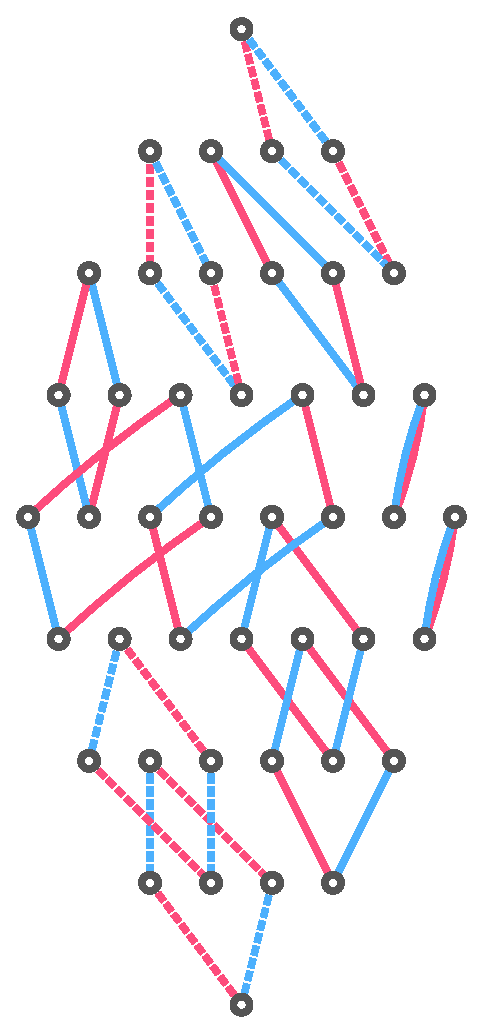
\includegraphics[width=0.3\textwidth]{resources/d4_s3s4}
		\caption{$Wk(\id)$ on the involutions in the Coxeter group $D_4$ with only $s_1,s_2$ edges on the left and only $s_3,s_4$ edges on the right side}
		\label{fig:d4_s1s2-and-d4_s3s4}
	\end{figure}
\end{exam}